\section{Model Origin: A Non-Significant, Under-Powered Moderation}
\label{sec:origin}

The project began with a model-\emph{origin} hypothesis---does the national/training origin
of a model (``CN-origin'' vs ``Western-origin'') moderate cooperation? We deliberately
\textbf{demote} this to a bounded case study, for two reasons: ``origin'' is a confounded
proxy (\S\ref{sec:apparatus}), and our own data show the channel dwarfs it. We are explicit
that the origin null is \emph{non-significant and under-powered}, not an established
equivalence.

\paragraph{The channel explains $\sim$20$\times$ more variance than origin (A3, \tC).}
A factorial decomposition of cooperation lock-in attributes
$\eta^2_{\text{channel}}=0.54$ to the communication rung and only
$\eta^2_{\text{origin}}=0.03$ to the origin grouping---roughly a $20\times$ difference. The
largest spread in cooperation is \emph{within} origin groups, not between them
(Figure~\ref{fig:f5}): two cross-origin pairs sit at opposite extremes of the per-pair
channel slope. The axis that organizes behavior is the affordance ladder, not pair
identity.

\paragraph{We cannot declare equivalence: the moderation is non-significant and
under-powered.}
We do \emph{not} claim ``origin doesn't matter'' in general, and---correcting an earlier
draft---we do \emph{not} claim a passed equivalence test. Operationalizing the powered null as
the per-pair channel effect (mean coop at L2/L3 minus L0/L1), the same-origin channel effect is
$0.688$ and the cross-origin effect is $0.517$; the observed moderation is $+0.171$ with a
non-significant Welch test ($p{=}0.090$). A two one-sided test (TOST) for equivalence
\textbf{does not pass} at any defensible bound (smallest $p_{\text{TOST}}\ge0.20$;
Appendix~\ref{app:a3}): with $10$ pairs per cell the point estimate sits too close to the bound,
so the data \emph{cannot} earn a tight equivalence claim. What the data \emph{do} support is
(a) \emph{no significant moderation}, and (b) a large, same-signed channel effect in \emph{both}
groups ($0.69$ vs.\ $0.52$). The honest statement is therefore \emph{``within these four models,
in English, with this scaffold, origin is a weaker driver than the channel, and the moderation
is not statistically distinguishable from zero---but our $n$ cannot rule out a moderate
effect.''} This is a within-sample case study, not a population claim about model nationality,
and explicitly not an equivalence result.

\paragraph{What actually varies: a DeepSeek-partner effect (\tE).}
The apparent ``origin'' signal that does exist is better explained by
\emph{individual-model cooperability} than by nationality. The two lowest-cooperation pairs
both \emph{contain DeepSeek-V3}: pairs including DeepSeek-V3 lock in at $\approx0.275$ at
L2/L3, versus $\approx0.85$ for DeepSeek-free pairs. This is a per-model partner effect that
cuts \emph{across} the origin grouping (DeepSeek-V3 was itself labeled ``CN-origin'' but the
matched-origin Qwen pairs cooperate readily). Attributing the spread to ``origin'' would
mislabel a single-model idiosyncrasy as a national-origin law---precisely the inference the
demotion is designed to avoid.

\begin{figure}[t]
\centering
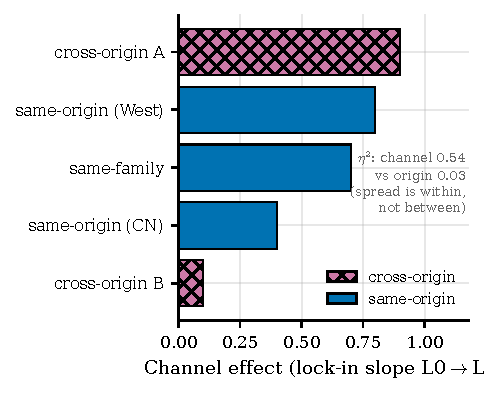
\includegraphics[width=\columnwidth]{figures/f5_a3_origin.pdf}
\caption{\textbf{A3 \tC{}: the channel, not model origin, drives cooperation.} Per-pair
channel effect (lock-in slope L0$\to$L3), colored by origin. Channel $\eta^2=0.54$ vs origin
$\eta^2=0.03$ ($\sim$20$\times$); the largest spread is \emph{within} origin groups, with two
cross-origin pairs at opposite extremes. The origin moderation is non-significant
($p{=}0.090$) and under-powered---not a passed equivalence test.}
\label{fig:f5}
\end{figure}
